\documentclass[12pt]{article}

% --- Encoding and languages ---
\usepackage[utf8]{inputenc}
\usepackage[english]{babel}

% --- Mathematics and symbols ---
\usepackage{amsmath, amsthm, amssymb}

% --- Layout and typography ---
\usepackage[left=3cm, right=3cm, top=3cm, bottom=3cm]{geometry}
\usepackage{setspace}
\usepackage{indentfirst}
\onehalfspacing

% --- Graphics and figures ---
\usepackage{graphicx}
\usepackage{subcaption}
\usepackage{tikz}

% --- Colors, links, urls ---
\usepackage{color}
\usepackage{url}
\usepackage{hyperref}

% --- Tables ---
\usepackage{array}
\usepackage{multirow}
\usepackage{siunitx}
\sisetup{output-decimal-marker = {.}}

% Easily centered p{} column:
\newcolumntype{C}[1]{>{\centering\arraybackslash}p{#1}}

% --- Lists ---
\usepackage{paralist}

% --- Source code ---
% NOTE: requires -shell-escape on Overleaf
\usepackage{minted}
\setminted[julia]{
  linenos=true,
  breaklines=true,
  encoding=utf8,
  frame=lines,
  framerule=0.5pt,
  autogobble,
  fontsize=\scriptsize,
}

% --- Algorithms ---
\usepackage[english,vlined,ruled,linesnumbered,boxruled]{algorithm2e}

% --- ABNT citations ---
\usepackage[alf]{abntex2cite}

% --- Link colors and PDF metadata ---
\definecolor{dark-red}{rgb}{0.4,0.15,0.15}
\definecolor{dark-blue}{rgb}{0.15,0.15,0.4}
\definecolor{medium-blue}{rgb}{0,0,0.5}
\hypersetup{
   colorlinks=true,
   linkcolor={dark-red},
   citecolor={dark-blue},
   urlcolor={medium-blue},
   pdfsubject={PGC III Report},
   pdfauthor={Ivan Zanutto Bastos, Matheus Pacheco de Oliveira},
   pdftitle={Neural Controller for Quadcopter Drones Developed via Genetic Algorithms}
}

% --- Useful macros ---
\newcommand{\up}[1]{\raisebox{1.5ex}[0pt]{#1}}
\newcommand{\HRule}{\rule{\linewidth}{0.5mm}}

% --- Theorems ---
\newtheorem{theorem}{Theorem}
\newtheorem{lemma}[theorem]{Lemma}
\newtheorem{proposition}[theorem]{Proposition}
\newtheorem{corollary}[theorem]{Corollary}
\theoremstyle{definition}
\newtheorem{definition}{Definition}


\begin{document}

% Title page
\thispagestyle{empty}
\begin{center}
    \textsc{Universidade Federal do ABC}\\[1em]
    
    \vfill

    \HRule \\[0.2cm]
    {\Large\bfseries Neural Controller for Quadcopter Drones Developed via Genetic Algorithms}\\
    
    \HRule \\[1.5cm]
    \vfill
    
    \begin{minipage}{0.4\textwidth}
    \begin{flushleft}
    \emph{Authors:}\\
    Ivan Zanutto Bastos \\
    Matheus Pacheco de Oliveira\\
    \end{flushleft}
    \end{minipage}
    \begin{minipage}{0.5\textwidth}
    \begin{flushright}
    \emph{RA:}\\
    11007116 \\
    11201722352 \\
    \end{flushright}
    \end{minipage}

    \vfill
    Advisor: Hugo Puertas de Araújo

    April/2025
\end{center}
\newpage

% Abstract
\begin{abstract}
The rapid technological advancements have driven the adoption of autonomous drones across various fields, notably in precision agriculture, logistics, and disaster management, where these devices provide increased efficiency and scalability compared to human-operated systems. In this context, artificial neural networks emerge as a promising solution due to their ability to adapt to dynamic and nonlinear environments. Simultaneously, genetic algorithms (GAs) have proven effective in optimizing neural networks by efficiently exploring solution spaces to adjust weights and parameters.

This study proposes the development of a neural controller for quadcopter drones using GAs, focusing on autonomous navigation in simulated environments. The controller is trained to navigate the drone to designated locations, assuming continuous flight without addressing takeoff or landing. To achieve this, a virtual environment was modeled using the Gymnasium platform, a neural network was implemented for drone control, and genetic algorithms were applied to optimize the controller.
\end{abstract}
\newpage

\section{Introduction}
In recent years, there has been a significant growth in research related to the development and application of drones in various areas, with a focus on the use of autonomous drones. These devices have proven to be particularly promising as they offer a substantial reduction in operational costs and greater scalability compared to operations that require human intervention. Among the main areas of application, precision agriculture stands out, where drones are used for crop monitoring and input spraying; delivery services, which promise greater logistical efficiency by reaching hard-to-access areas; and disaster management, where the speed and accuracy of drones are essential for mapping affected areas, assisting search and rescue operations, and assessing damage.~\cite{Agriculture, DeliverySystem, DisasterManagement}.

In this context, artificial neural networks (ANNs) emerge as a promising solution due to their capacity to learn and generalize complex behaviors from training data, without the need for explicit system models. These networks, inspired by the functioning of the human brain, are particularly effective in dynamic and non-linear environments, where operating variables and conditions can change rapidly. These characteristics make neural networks a powerful tool for developing flight controllers that need to continuously adapt to environmental variables, such as wind or unexpected obstacles.~\cite{AutonomousDroneRL}.

In parallel, the use of Genetic Algorithms (GAs) has proven to be a promising approach for training neural networks. Inspired by the processes of natural selection, GAs are powerful tools for the optimization of parameters in complex systems, such as those involved in adjusting the weights of a neural network. They allow for the efficient exploration of the solution space, finding network configurations that maximize drone performance in different scenarios.~\cite{ReviewGeneticAlgorithm, GeneticAlgorithms}.

Therefore, this work proposes the combination of neural networks and genetic algorithms as a robust and adaptable solution for the development of an autonomous drone flight controller, with the potential to overcome challenges present in critical applications.

\section{Objectives}
\subsection{General Objective}
Develop a neural controller for quadcopter drones using genetic algorithms, capable of autonomous navigation in a virtual environment, moving to a designated target. The controller assumes continuous flight; takeoff and landing are out of scope.

\subsection{Specific Objectives}
\begin{enumerate}
    \item \textbf{Virtual Environment:} Design and implement a Gymnasium-based environment to reproduce and visualize drone behavior.
    \item \textbf{Neural Network:} Design and implement an artificial neural network for drone control in simulation.
    \item \textbf{Genetic Algorithms:} Optimize the controller by tuning parameters and, when applicable, topology.
    \item \textbf{Simulation and Evaluation:} Assess navigation and obstacle avoidance performance in simulation.
\end{enumerate}

\section{Proposed Approach}
The project will commence with the modeling of the simulated environment using Gymnasium, an open-source Python library. This environment will be 3-dimensional and configured to include a variety of obstacles and destinations for the drone. It will also define the model quality parameters necessary to calculate our fitness function, thus offering a robust test scenario for the controller.

The neural network will initially be designed with a simple architecture, tailored to handle the real-time control of the drone. The network structure will include inputs corresponding to the drone's sensors (such as distances to obstacles and relative position to the destination) and outputs that will map to the control commands, such as propeller activation and speed.

Genetic Algorithms will be employed to train the neural network, starting with an initial population of networks with random parameters. The performance of each individual will be evaluated based on the drone's ability to reach the destination, or how close it gets, without colliding with obstacles. The fittest individuals will be selected for reproduction, applying genetic operators such as crossover and mutation to generate the next generation of neural networks. This process will be repeated until the controller achieves a desirable performance or until a maximum number of generations is reached.

Finally, the performance of the trained controller will be evaluated in a series of simulated tests. The drone's success in various environment configurations will be verified.

\section{Methodology}
\subsection{Simulated Environment}
The environment was built on top of the \textit{gym-pybullet-drones} project \cite{panerati2021learning}, which uses the \textit{PyBullet} library \cite{coumans2019} for physics simulation and the \textit{Crazyflie 2.0} \cite{forster2015system} as the drone model. The main properties of the environment and the changes made to adapt it to the requirements of this work are detailed below.

\subsubsection{Observation Space}
The neural network observation space was defined as: Relative position to the target (via GPS), velocity (via GPS), acceleration (via accelerometer), orientation quaternion (via gyroscope), depth map (via LIDAR), and altitude (via distance sensor).

\subsubsection{Action Space}
The action space consists of 4 values ranging from $-1$ to $1$ that control the rotation of each motor individually according to:
\[
\text{rpm}(x) = h (1 + 0.05x)
\]
where $h$ is the rotation required to keep the drone hovering in place.

\subsubsection{Non-conservative Forces}
\textit{PyBullet} has a property called \textit{damping}, which acts as a global friction term for all objects in the simulation. It works as follows:
\[
a_d = -d_v v
\text{, and }
\alpha_d = -d_\omega \omega
\]
where $a_d$ is the linear acceleration caused by the \textit{damping}, $d_v$ is the linear \textit{damping}, and $v$ is the linear velocity. The angular terms are defined analogously. \newline
By default, $d_v = d_\omega = 0.04$. However, the base project \textit{gym-pybullet-drones} includes a drag implementation based on experimental data, which was used instead of the linear \textit{damping}. The angular \textit{damping} was not modified.

\subsubsection{Termination and Truncation Criteria}
The episode is considered successful if the distance from the drone to the goal reaches the threshold of $0.5$ meters. \newline
The episode is truncated if the drone’s tilt exceeds the threshold of $0.4$ radians or if the distance to the goal exceeds $\sqrt{2}$ times the initial distance.

\subsubsection{Fitness Function}
Initially, only the distance to the goal was used as an attribute of the \textit{fitness} function, given by:
\[
F_d(d)=
\begin{cases}
     1 - (d/D)^2, & \text{if } d \leq D\\
     0,           & \text{otherwise}
\end{cases}
\]
\begin{center}
    where $d$ is the final distance and $D$ is the initial distance.
\end{center}
However, to ensure that the drone actually stops at the goal and to encourage trajectory efficiency, the final velocity and total duration were added as attributes. Thus, the final function used is:
\[
F(d, v, t)=
\begin{cases}
     50 \times F_d(d),                                       & \text{if } d \geq \frac{\sqrt{2}}{2}\\
     50 \times F_d(d) + 30 \times F_v(v),                    & \text{if } d < \frac{\sqrt{2}}{2} \text{ and } v \geq 1\\
     50 \times F_d(d) + 30 \times F_v(v) + 20 \times F_t(t), & \text{otherwise}
\end{cases}
\]
where $FR_v$ and $F_t$ are given by:
\[
F_v(v)=1 - (v/V)^2
\]
\begin{center}
    where $v$ is the final velocity and $V$ is the maximum velocity.
\end{center}
\[
F_t(t)=1 - \left(\frac{t - T_{min}}{T_{max}-T_{min}}\right)^2
\]
\begin{center}
    where $t$ is the final time, $T_{max} = \frac{\text{initial distance}}{\text{minimum velocity}}$ and $T_{min} = \frac{\text{initial distance}}{\text{maximum velocity}}$. \newline
    The minimum velocity is defined as 1 m/s and the maximum velocity as 20 m/s.
\end{center}

This definition makes the \textit{fitness} work in tiers: velocity only becomes relevant when the distance is smaller than $\frac{\sqrt{2}}{2}$, and time only becomes relevant when the velocity is lower than 1. The values were chosen based on the success threshold ($0.5$). The idea behind this approach is to impose a priority order on the attributes, which prevents competition between them and speeds up convergence.

Furthermore, the function now ranges from 0 to 100, instead of 0 to 1, to make visualization easier: 50 points are related to distance, 30 to velocity, and 20 to time. These values were chosen according to the importance of each attribute with respect to the desired outcome.

\subsection{Genetic Algorithms with DEAP}
We first experimented with PyGAD (\textit{Python Genetic Algorithm})~\cite{DBLP:journals/corr/abs-2106-06158}. We then adopted DEAP (\textit{Distributed Evolutionary Algorithms in Python})~\cite{DEAP_JMLR2012} for greater flexibility in more complex evolutionary setups.

\subsubsection{Hyperparameters}
The GA explores the following hyperparameters:
\begin{itemize}
    \item Minimum/maximum number of hidden layers
    \item Minimum/maximum neurons per hidden layer
    \item Population size
    \item Number of generations
    \item Crossover rate
    \item Mutation rates
    \item Tournament size
\end{itemize}

\subsubsection{Individual Representation}
The chromosome has fixed length based on the allowed range of hidden layers. Some genes may be inactive depending on the chosen topology. Gene semantics:
\begin{itemize}
    \item Index 0: number of hidden layers (bounded by hyperparameters)
    \item Indices $i=1$ to $i=\textit{max hidden layers}$: neurons in hidden layer $i$ (bounded)
    \item Remaining genes: synaptic weights. Each layer occupies predetermined index ranges up to the maximum number of weights per layer, computed from the maximum neurons per layer.
\end{itemize}

\subsubsection{Algorithm}
We first used \texttt{deap.algorithms.eaSimple()}, the standard evolutionary loop: evaluate each individual, apply tournament selection, then crossover and mutation. The chromosome encodes both topology and weights.

We also tested a coevolutionary variant with two populations:
\begin{enumerate}
    \item A topology population evolved while fixing the best weights.
    \item A weight population evolved while fixing the best topology.
\end{enumerate}
At each macro-generation, the topology population evolves for three micro-generations using the best weights; then the weight population evolves for three micro-generations using the best topology.

\subsection{Genetic Neuroevolution with NEAT}
We additionally used \textit{neat-python}~\cite{McIntyre_neat-python}, which implements \textit{NeuroEvolution of Augmenting Topologies} (NEAT)~\cite{neat_original}. NEAT starts from a minimal topology (inputs and outputs) and adds neurons and connections by mutation.

\subsubsection{Genome Representation}
Genes represent nodes (neurons) or connections and include:
\begin{enumerate}
    \item Innovation number (historical marker)
    \item Synaptic weight
    \item Enabled/disabled flag
    \item If connection: the two endpoint nodes
    \item If node: activation function
\end{enumerate}

\subsubsection{Mutation}
Each generation, mutations may:
\begin{enumerate}
    \item Perturb synaptic weights
    \item Add a connection
    \item Add a node
    \item Change activation function (not in the output layer)
    \item Enable or disable a connection
\end{enumerate}
New nodes and connections receive new innovation numbers, which support consistent gene alignment during crossover and enable speciation.

\subsubsection{Crossover}
Parent genes are aligned by innovation number and classified as:
\begin{enumerate}
  \item \textbf{Matching genes:} present in both parents.
  \item \textbf{Disjoint genes:} present in only one parent, with innovation $\le$ the other parent’s maximum.
  \item \textbf{Excess genes:} present in only one parent, with innovation $>$ the other parent’s maximum.
\end{enumerate}
Matching genes inherit weights from either parent at random; disjoint and excess genes are copied from the more fit parent (or from both in a tie).

\subsubsection{Speciation}
This algorithm also introduces the idea of \textbf{speciation} to protect new innovations, since a new node can, for instance, worsen the \textit{fitness} in the short term, but become useful in the long run after its weight has evolved over several generations.

To this end, the notion of a compatibility distance, $\delta$, between two different genomes is introduced, representing how different these two organisms are. If this distance is above a given threshold, $\delta_t$, the two organisms are considered to belong to different species.

\[
\delta = \frac{c_1E}{N} + \frac{c_2D}{N} + c_3\overline{W}
\]

Where,

\begin{itemize}[]
    \item $E$: Number of excess genes
    \item $D$: Number of disjoint genes
    \item $\overline{W}$: Average difference of synaptic weights
    \item $N$: Size of the larger genome
    \item $ c_1, c_2, c_3$: Tunable coefficients
\end{itemize}

To protect new innovations, the \textit{fitness} of each organism is adjusted by dividing it by the size of its species. This penalizes large species and prevents a single species from dominating the entire population, while also giving new mutations time to develop.

Moreover, species are completely eliminated if they fail to improve within a given period (in this case, 15 generations), except for the three best species, which are protected by elitism to avoid a total wipeout of the population.

Finally, to allocate offspring, each species is first assigned a number of descendants proportional to the sum of the adjusted \textit{fitness} of all its organisms. Then, the worst-performing organisms are removed and the remaining ones reproduce. The entire population of each species is replaced by its offspring, with the exception of the organisms protected by elitism (2 per species).

\section{Results}
Initial experiments used a fixed target position and compared three approaches:
\begin{enumerate}
    \item DEAP — single population
    \item DEAP — coevolution with separate topology and weight populations
    \item NEAT
\end{enumerate}
The input layer had 14 neurons (matching the observation space), and the output layer had 4 neurons with $\tanh$ activation, one per motor, each in $[-1,\,1]$.

Further hyperparameter exploration is warranted and would require additional compute.

\subsection{DEAP — Single Population}
As shown in Fig.~\ref{fig:primeiro_fitness_gens}, the algorithm raised mean fitness over generations, with occasional improvements in the best individual. It did not reach the optimum: the best fitness was \num{49.3}, close to the target but short of contact. Figure~\ref{fig:primeiro_topologia} shows premature convergence to a single hidden layer with \num{15} neurons.

This run used a population of 50. Networks could have from \num{1} to \num{10} hidden layers and \num{5} to \num{20} neurons per hidden layer. Mutation settings: \SI{10}{\percent} chance to change the number of layers, \SI{10}{\percent} chance to change the neuron count in a random layer, and Gaussian perturbations to synaptic weights.

\begin{figure}[htbp]
    \centering
    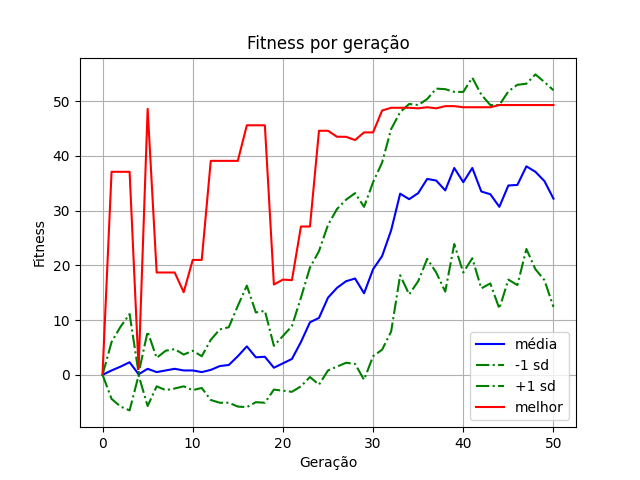
\includegraphics[width=0.8\textwidth]{imgs/deap_primeiro_algoritmo/fitness.png}
    \caption{Performance of the single-population DEAP algorithm: fitness per generation.}
    \label{fig:primeiro_fitness_gens}
\end{figure}

\begin{figure}[!htbp]
  \centering
  \begin{subfigure}[b]{0.48\textwidth}
    \centering
    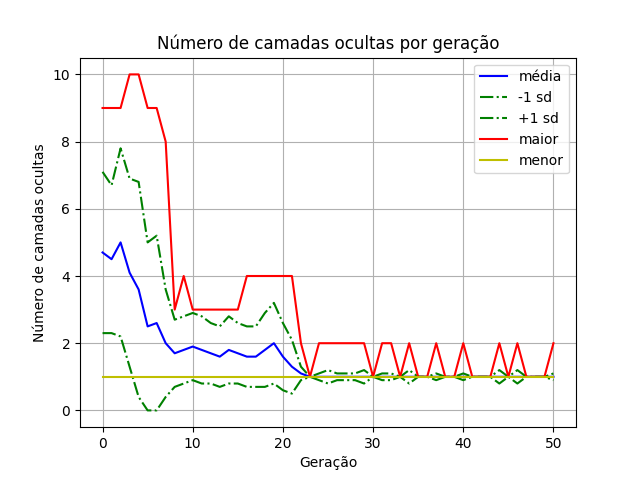
\includegraphics[width=\linewidth]{imgs/deap_primeiro_algoritmo/num_layers.png}
    \caption{Hidden-layer count evolution}
    \label{fig:sub1}
  \end{subfigure}
  \begin{subfigure}[b]{0.48\textwidth}
    \centering
    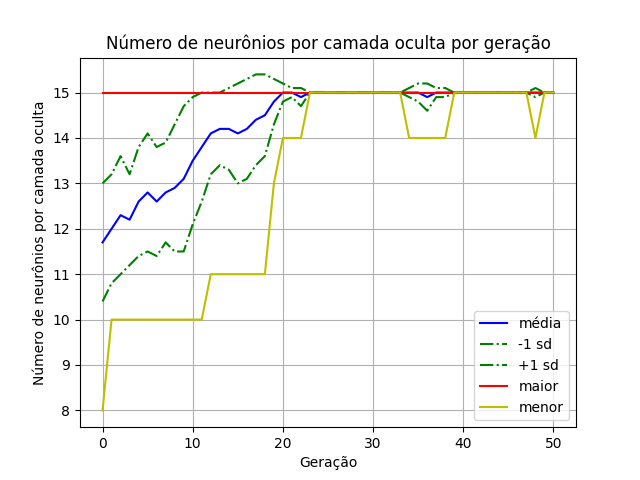
\includegraphics[width=\linewidth]{imgs/deap_primeiro_algoritmo/neurons.png}
    \caption{Hidden-layer neuron count evolution}
    \label{fig:sub2}
  \end{subfigure}
  \caption{Topology evolution with the single-population DEAP algorithm.}
  \label{fig:primeiro_topologia}
\end{figure}

\subsection{DEAP — Coevolution}
Figure~\ref{fig:fitness_gens} shows the coevolutionary setup (separate topology and weight populations), which achieved a best fitness of \num{58.2} and a mean of \num{34.9}. Each population had \num{500} individuals and \num{100} macro-generations, each comprising \num{3} topology micro-generations followed by \num{3} weight micro-generations. Elitism preserved \SI{10}{\percent} of the best parents.

\begin{figure}[htbp]
    \centering
    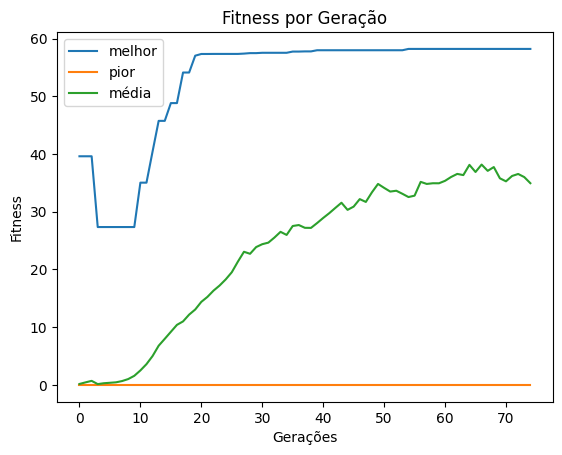
\includegraphics[width=0.8\textwidth]{imgs/fitness_gens.png}
    \caption{Coevolutionary algorithm: fitness per generation.}
    \label{fig:fitness_gens}
\end{figure}

\subsection{NEAT}
Because NEAT uses a compact internal network representation (without \textit{keras}/\textit{pytorch} overhead), runs were faster, enabling larger populations and broader sweeps. We used a population of 1500; activation choices included \textit{sigmoid}, \textit{ReLU}, and \textit{tanh}.

In Fig.~\ref{fig:neat_fitness_gens}, fitness increases steadily, reaching a maximum of \num{98.49}. The drone reached and stopped at the target; the remaining gap to the theoretical maximum (\num{100}) reflects travel time. Figure~\ref{fig:neat_fitness_gens_começo} zooms into the first 100 generations: rapid gains until roughly generation 20, followed by occasional improvements from mutation.

\begin{figure}[htbp]
    \centering
    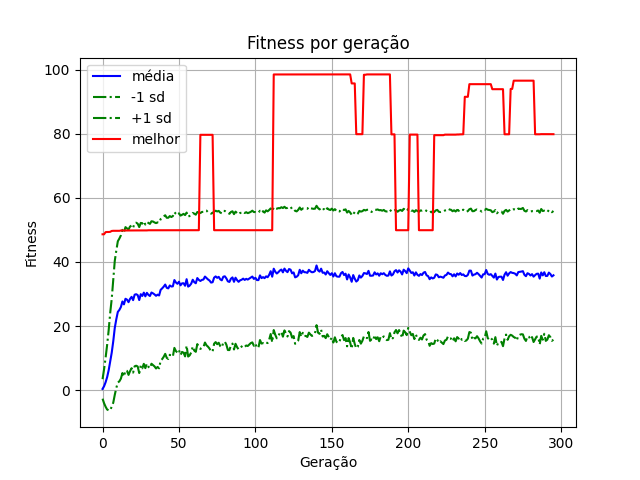
\includegraphics[width=0.8\textwidth]{imgs/neat/fitness.png}
    \caption{NEAT performance: fitness per generation.}
    \label{fig:neat_fitness_gens}
\end{figure}

\begin{figure}[htbp]
    \centering
    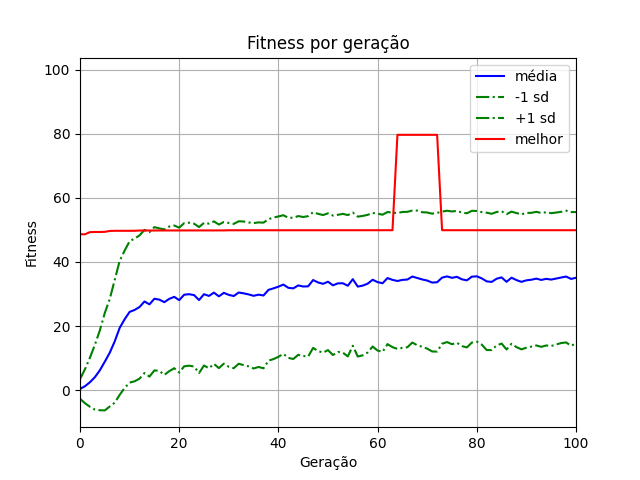
\includegraphics[width=0.8\textwidth]{imgs/neat/fitness_começo.png}
    \caption{NEAT: fitness over the first 100 generations.}
    \label{fig:neat_fitness_gens_começo}
\end{figure}

Figure~\ref{fig:neat_especiacao} illustrates speciation dynamics. Panel~\ref{fig:species} shows species sizes (min/mean/max per generation); Panel~\ref{fig:number_species} shows the number of species per generation.

\begin{figure}[!htbp]
  \centering
  \begin{subfigure}[b]{0.48\textwidth}
    \centering
    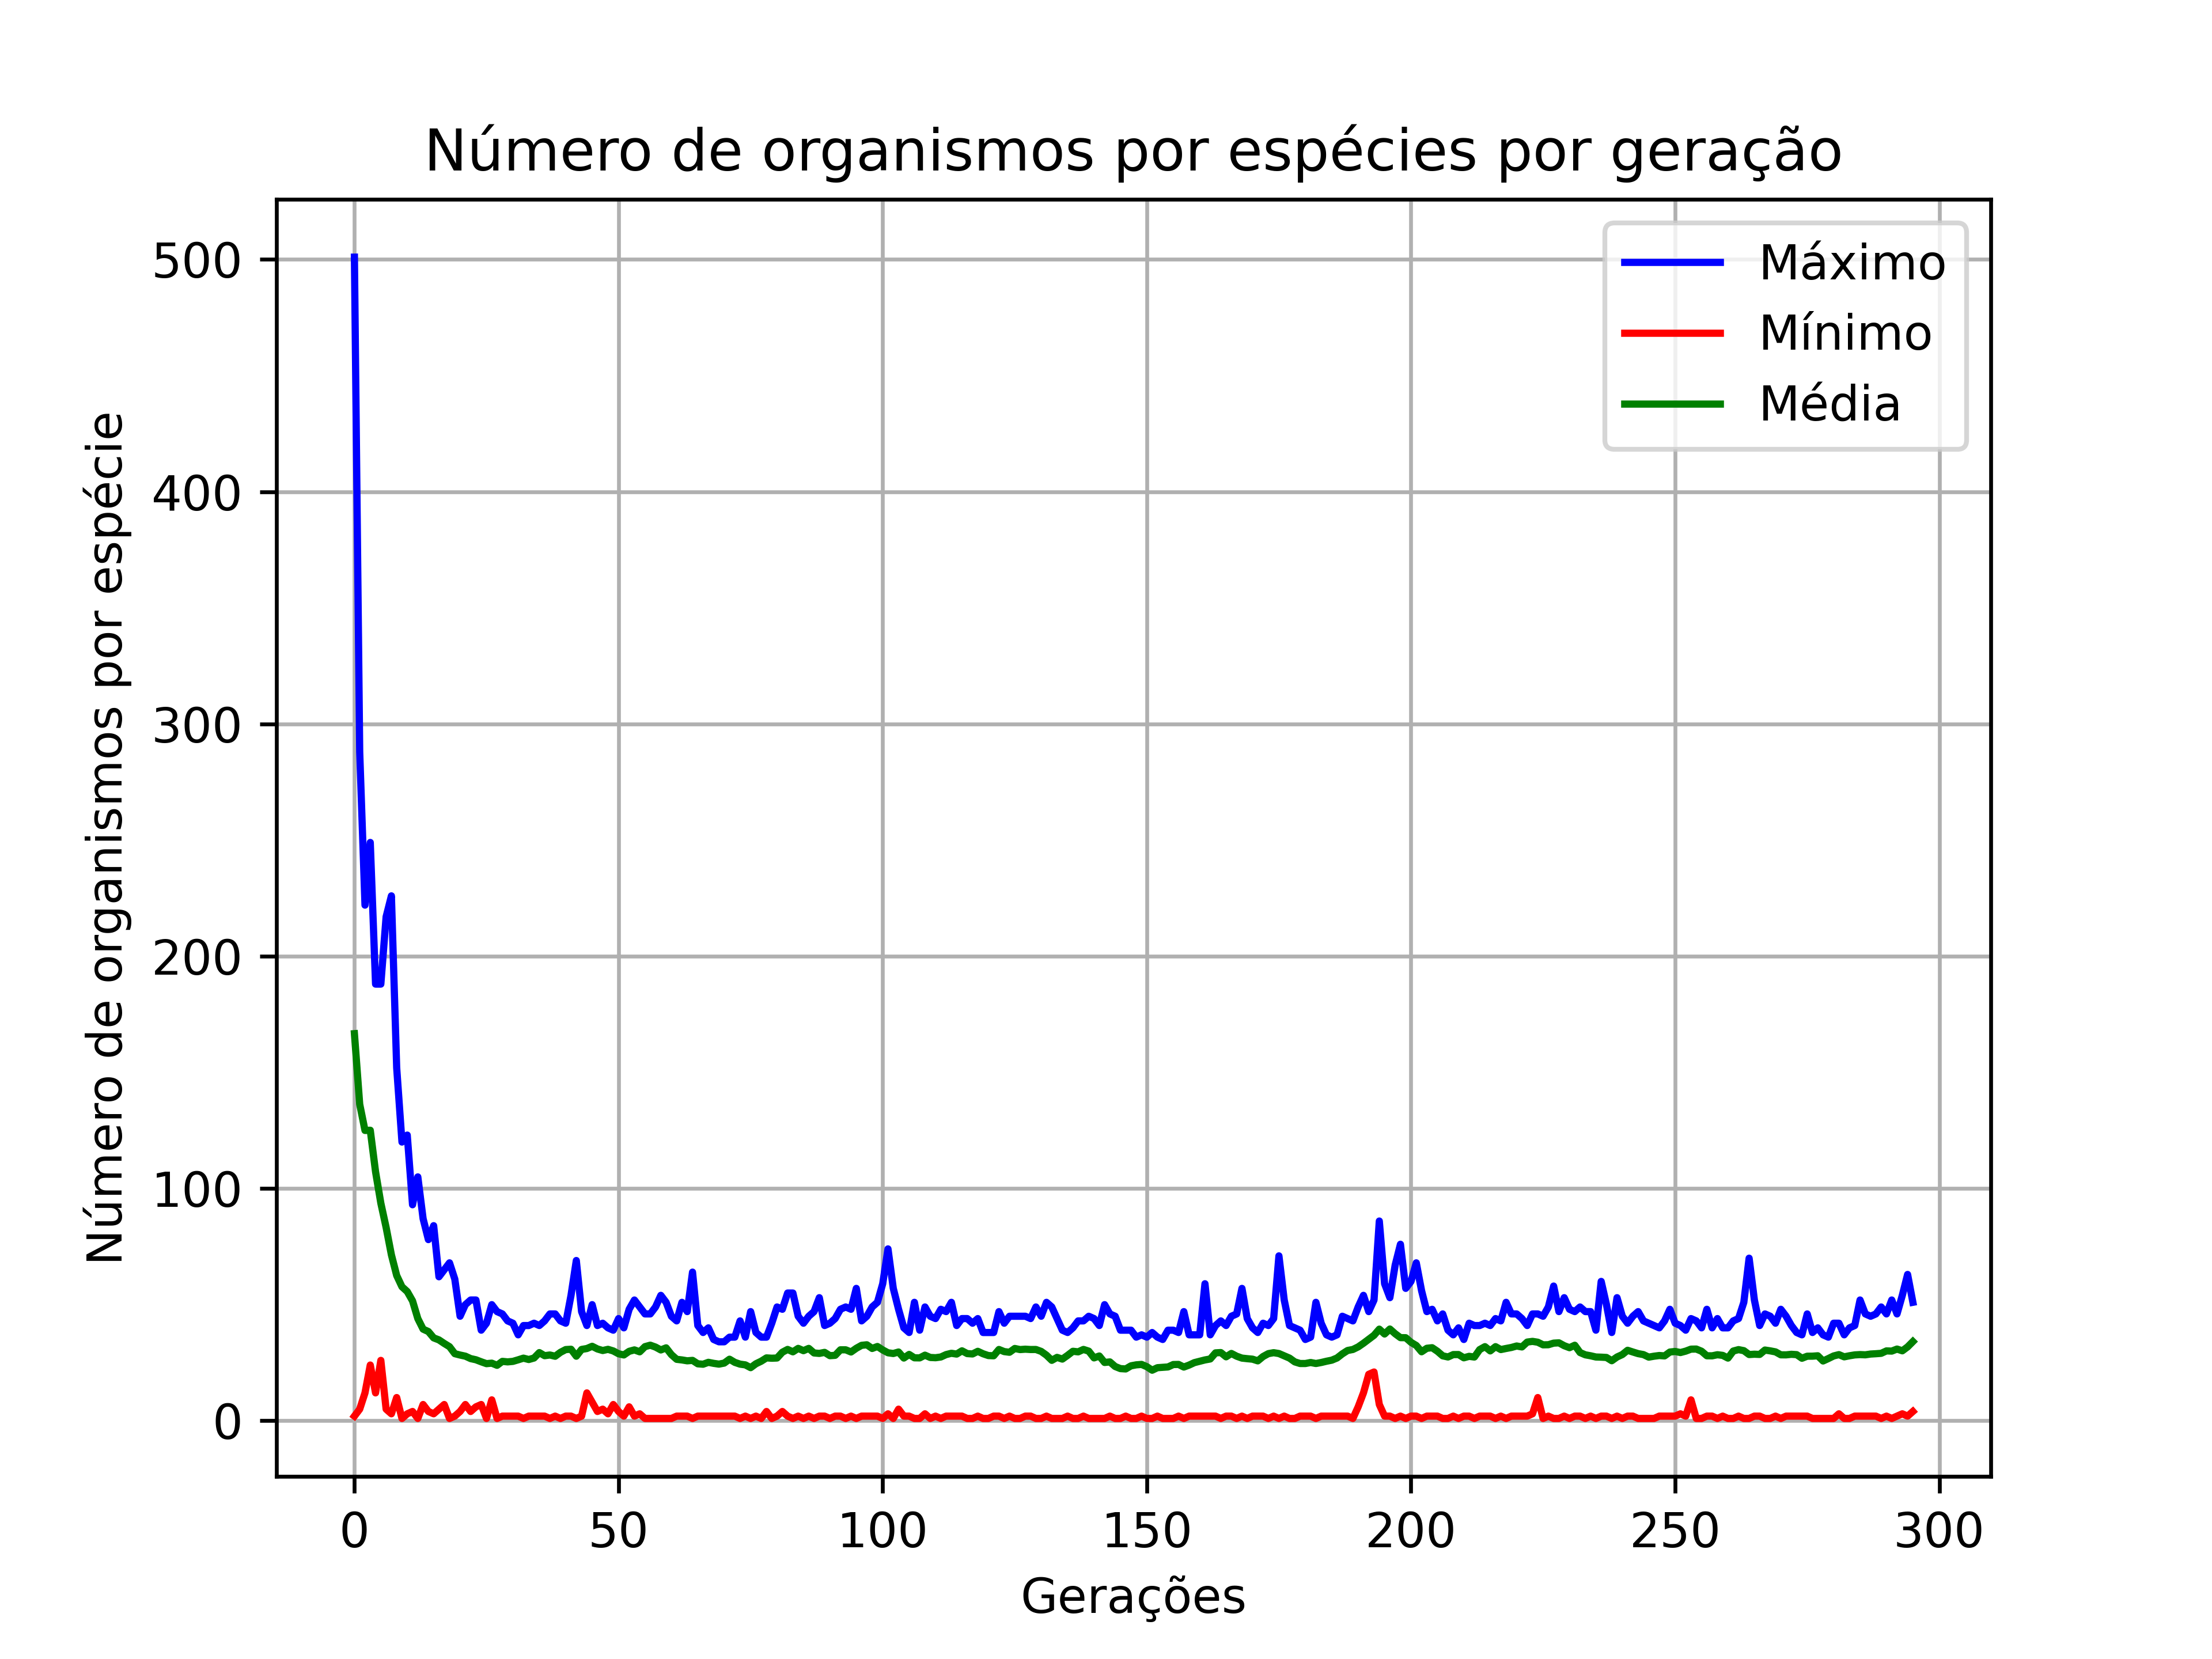
\includegraphics[width=\linewidth]{imgs/neat/size_species.png}
    \caption{Species size per generation}
    \label{fig:species}
  \end{subfigure}
  \begin{subfigure}[b]{0.48\textwidth}
    \centering
    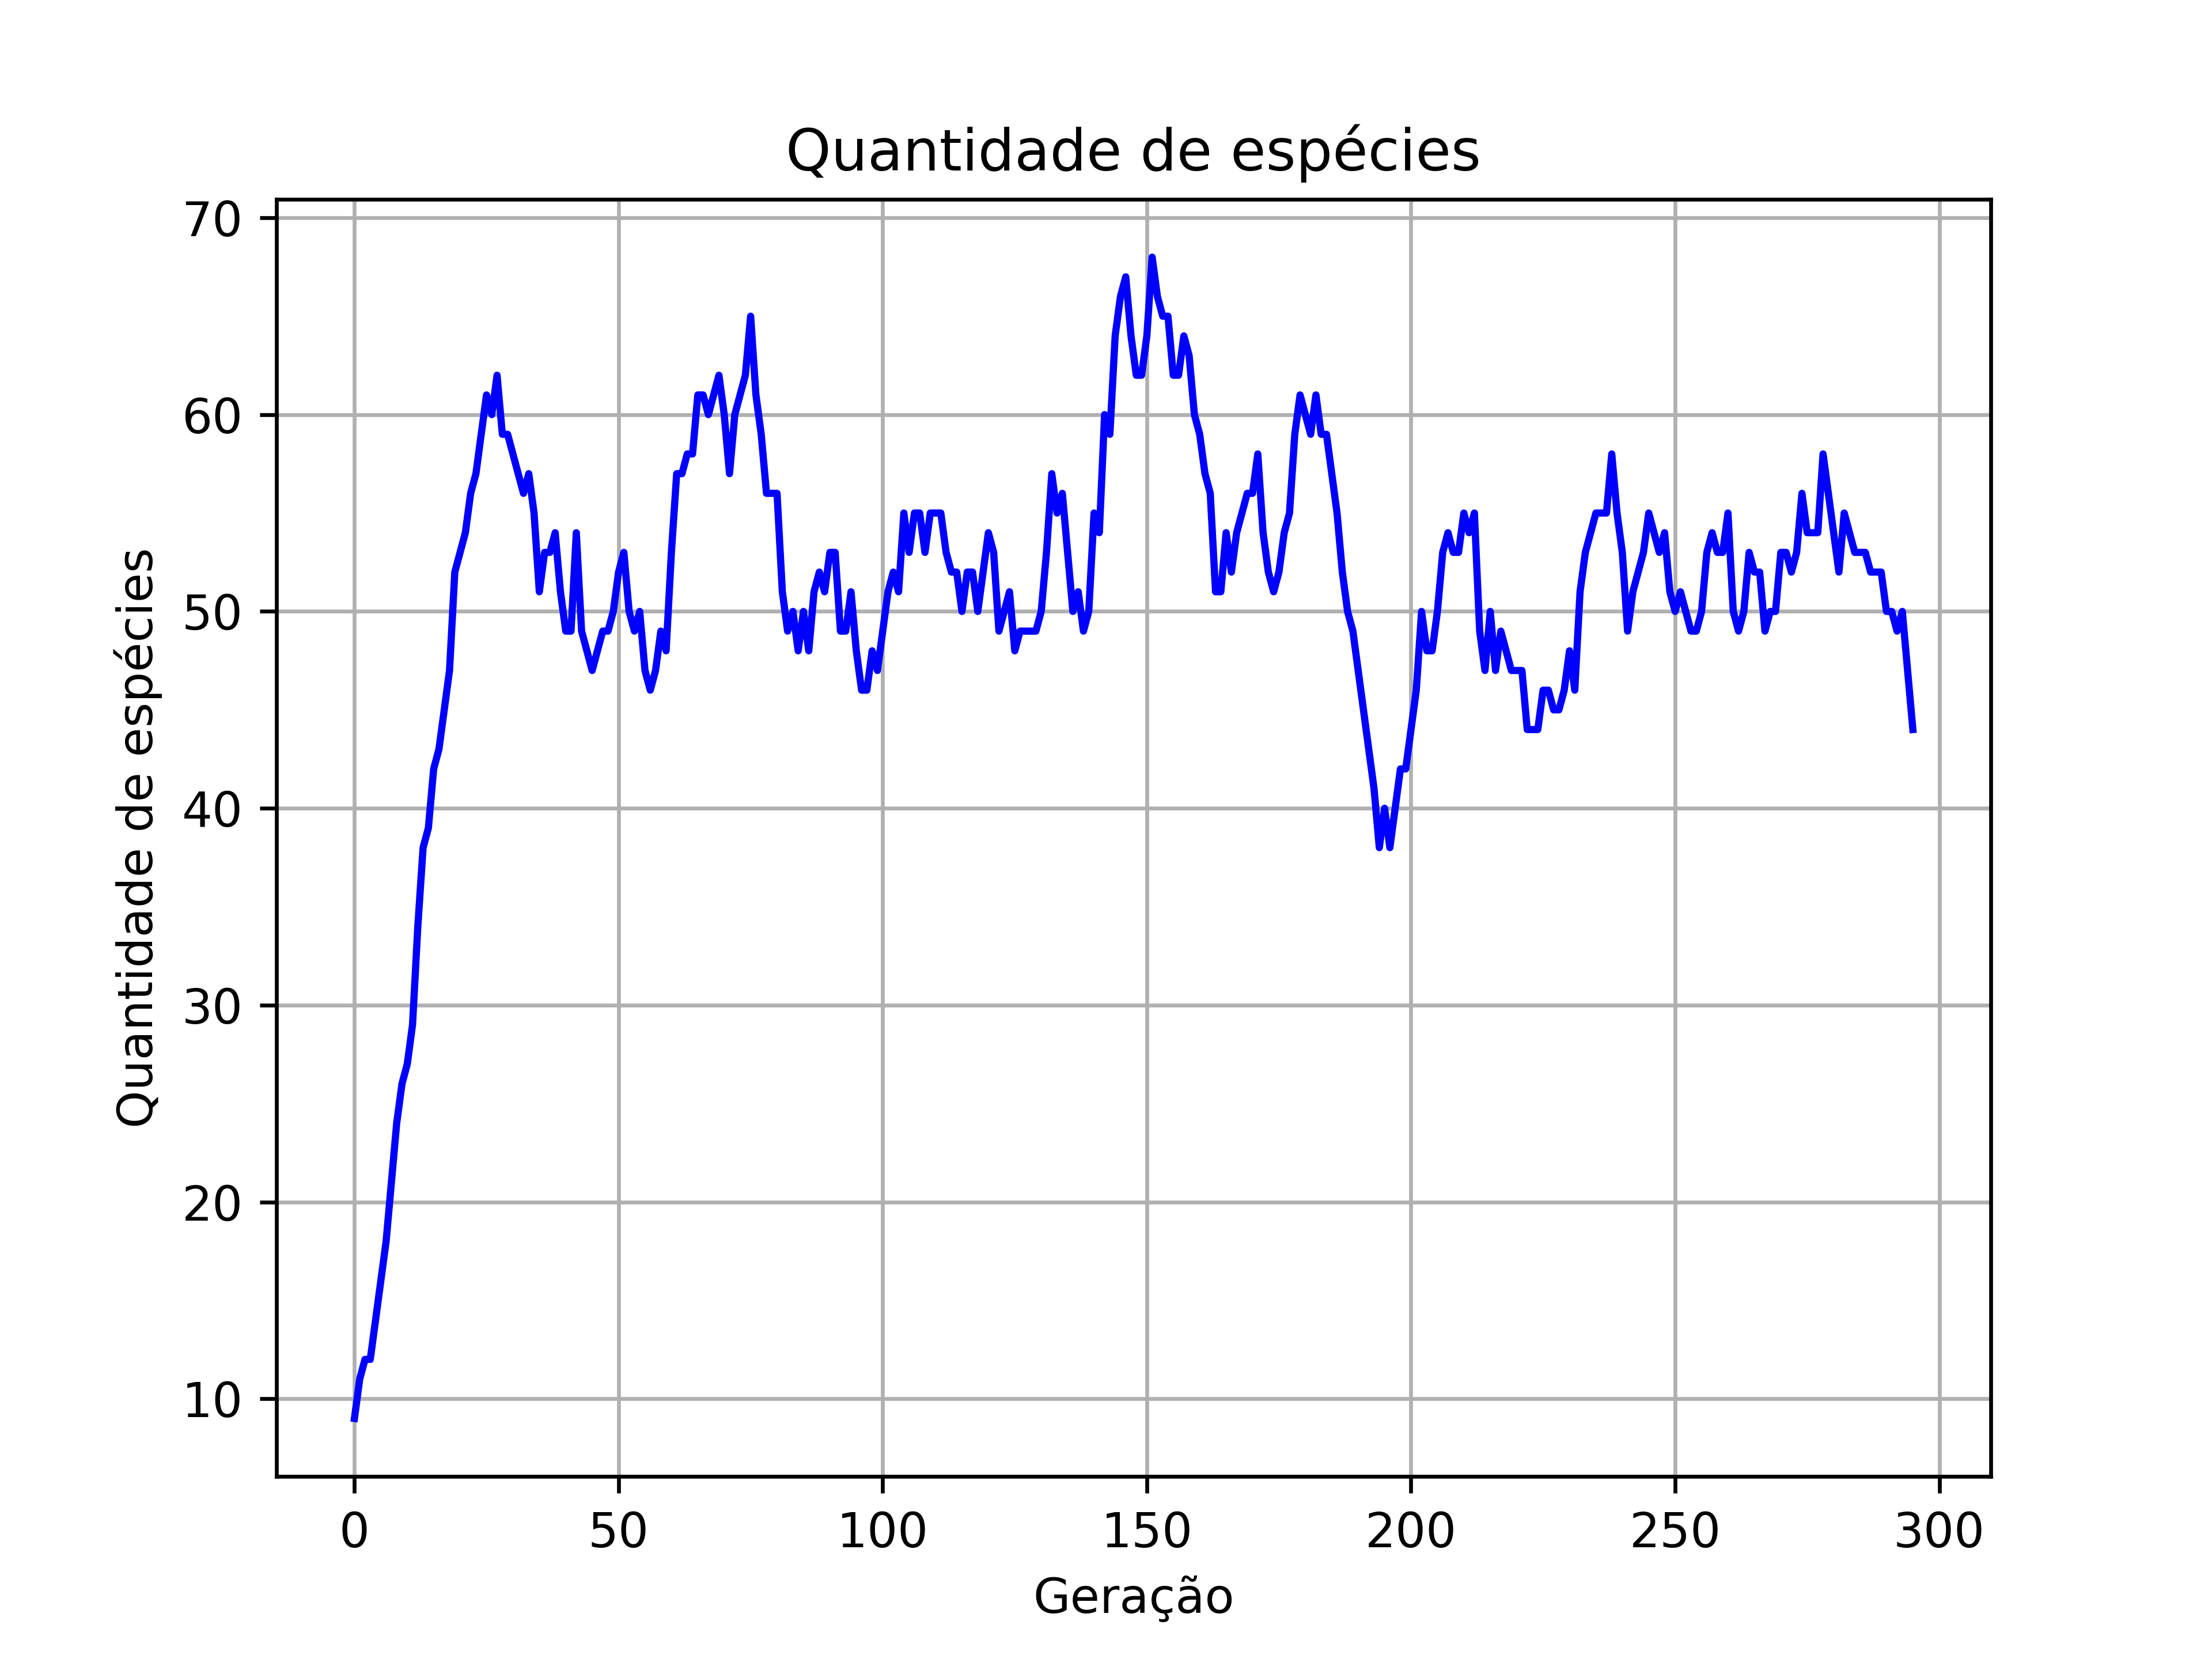
\includegraphics[width=\linewidth]{imgs/neat/number_species.png}
    \caption{Number of species per generation}
    \label{fig:number_species}
  \end{subfigure}
  \caption{Speciation dynamics (NEAT).}
  \label{fig:neat_especiacao}
\end{figure}

Finally, Fig.~\ref{fig:winner_net} depicts the highest-fitness network. Square nodes are inputs; round nodes indexed \num{0}–\num{3} are outputs; the remaining round nodes are hidden units. Green edges indicate positive weights and red edges negative weights; dashed edges are disabled connections. The winning network included two hidden neurons with \textit{ReLU} activation.

\begin{figure}[!htbp]
    \centering
    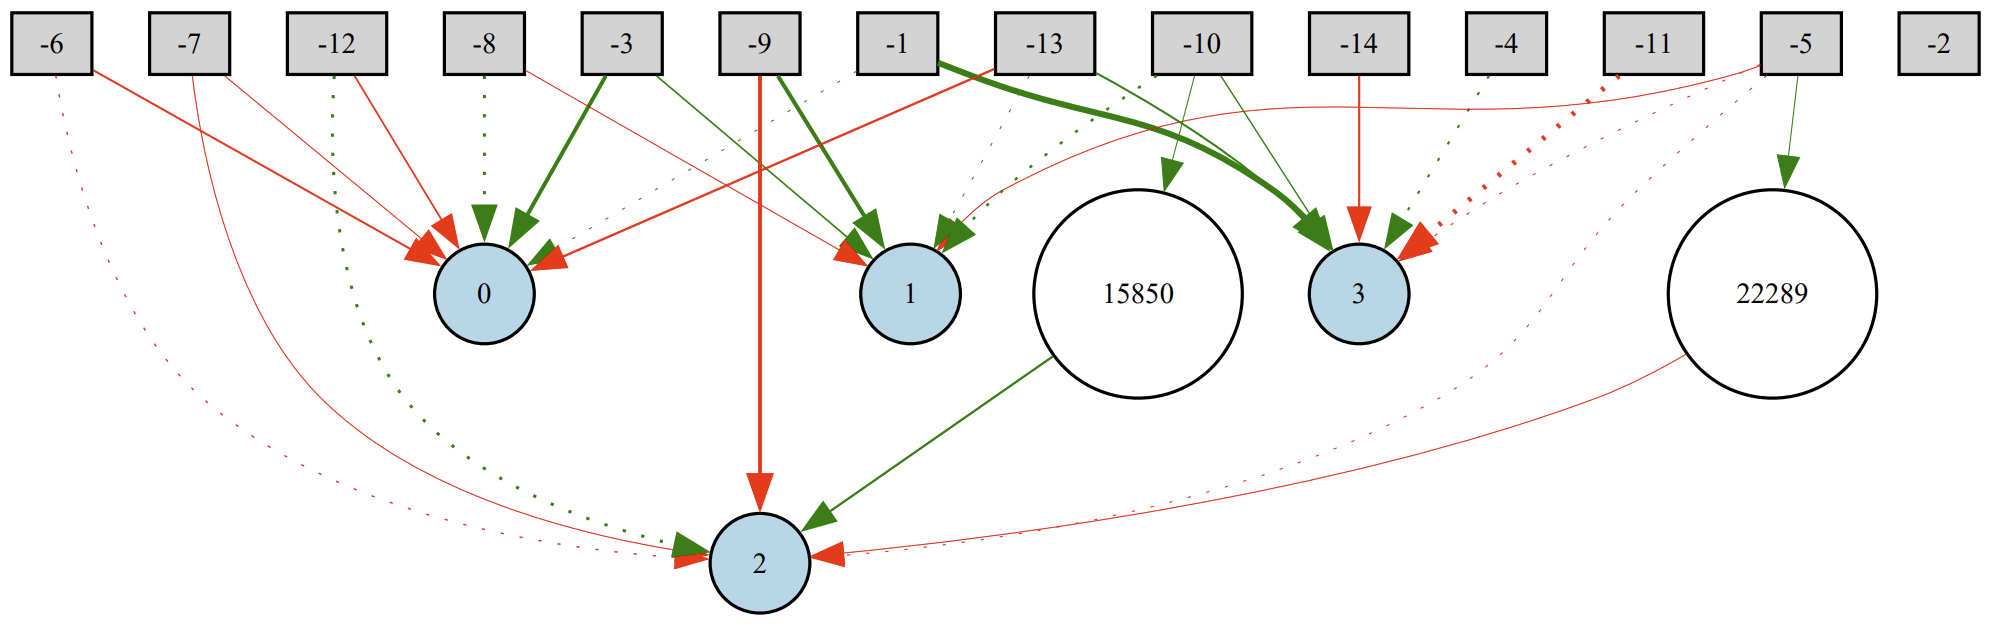
\includegraphics[width=0.8\textwidth]{imgs/neat/winner_net.png}
    \caption{Architecture of the best-performing network evolved by NEAT.}
    \label{fig:winner_net}
\end{figure}

\bibliography{bibliografia}

\end{document}

